%% bare_jrnl.tex
%% V1.4b
%% 2015/08/26
%% by Michael Shell
%% see http://www.michaelshell.org/
%% for current contact information.
%%
%% This is a skeleton file demonstrating the use of IEEEtran.cls
%% (requires IEEEtran.cls version 1.8b or later) with an IEEE
%% journal paper.
%%
%% Support sites:
%% http://www.michaelshell.org/tex/ieeetran/
%% http://www.ctan.org/pkg/ieeetran
%% and
%% http://www.ieee.org/

%%*************************************************************************
%% Legal Notice:
%% This code is offered as-is without any warranty either expressed or
%% implied; without even the implied warranty of MERCHANTABILITY or
%% FITNESS FOR A PARTICULAR PURPOSE! 
%% User assumes all risk.
%% In no event shall the IEEE or any contributor to this code be liable for
%% any damages or losses, including, but not limited to, incidental,
%% consequential, or any other damages, resulting from the use or misuse
%% of any information contained here.
%%
%% All comments are the opinions of their respective authors and are not
%% necessarily endorsed by the IEEE.
%%
%% This work is distributed under the LaTeX Project Public License (LPPL)
%% ( http://www.latex-project.org/ ) version 1.3, and may be freely used,
%% distributed and modified. A copy of the LPPL, version 1.3, is included
%% in the base LaTeX documentation of all distributions of LaTeX released
%% 2003/12/01 or later.
%% Retain all contribution notices and credits.
%% ** Modified files should be clearly indicated as such, including  **
%% ** renaming them and changing author support contact information. **
%%*************************************************************************


% *** Authors should verify (and, if needed, correct) their LaTeX system  ***
% *** with the testflow diagnostic prior to trusting their LaTeX platform ***
% *** with production work. The IEEE's font choices and paper sizes can   ***
% *** trigger bugs that do not appear when using other class files.       ***                        
% The testflow support page is at:
% http://www.michaelshell.org/tex/testflow/



\documentclass[journal]{IEEEtran}
%
% *** GRAPHICS RELATED PACKAGES ***
%
\usepackage{graphicx} 
\usepackage{subcaption} 
\ifCLASSINFOpdf
  % \usepackage[pdftex]{graphicx}
  % declare the path(s) where your graphic files are
  % \graphicspath{{../pdf/}{../jpeg/}}
  % and their extensions so you won't have to specify these with
  % every instance of \includegraphics
  % \DeclareGraphicsExtensions{.pdf,.jpeg,.png}
\else
  % or other class option (dvipsone, dvipdf, if not using dvips). graphicx
  % will default to the driver specified in the system graphics.cfg if no
  % driver is specified.
  % \usepackage[dvips]{graphicx}
  % declare the path(s) where your graphic files are
  % \graphicspath{{../eps/}}
  % and their extensions so you won't have to specify these with
  % every instance of \includegraphics
  % \DeclareGraphicsExtensions{.eps}
\fi
% graphicx was written by David Carlisle and Sebastian Rahtz. It is
% required if you want graphics, photos, etc. graphicx.sty is already
% installed on most LaTeX systems. The latest version and documentation
% can be obtained at: 
% http://www.ctan.org/pkg/graphicx
% Another good source of documentation is "Using Imported Graphics in
% LaTeX2e" by Keith Reckdahl which can be found at:
% http://www.ctan.org/pkg/epslatex
%
% latex, and pdflatex in dvi mode, support graphics in encapsulated
% postscript (.eps) format. pdflatex in pdf mode supports graphics
% in .pdf, .jpeg, .png and .mps (metapost) formats. Users should ensure
% that all non-photo figures use a vector format (.eps, .pdf, .mps) and
% not a bitmapped formats (.jpeg, .png). The IEEE frowns on bitmapped formats
% which can result in "jaggedy"/blurry rendering of lines and letters as
% well as large increases in file sizes.
%
% You can find documentation about the pdfTeX application at:
% http://www.tug.org/applications/pdftex


% correct bad hyphenation here
\hyphenation{op-tical net-works semi-conduc-tor}


\begin{document}
%
% paper title
% Titles are generally capitalized except for words such as a, an, and, as,
% at, but, by, for, in, nor, of, on, or, the, to and up, which are usually
% not capitalized unless they are the first or last word of the title.
% Linebreaks \\ can be used within to get better formatting as desired.
% Do not put math or special symbols in the title.
\title{Improving Sign Recognition Models with Blender-Synthesized Data}
%
%
% author names and IEEE memberships
% note positions of commas and nonbreaking spaces ( ~ ) LaTeX will not break
% a structure at a ~ so this keeps an author's name from being broken across
% two lines.
% use \thanks{} to gain access to the first footnote area
% a separate \thanks must be used for each paragraph as LaTeX2e's \thanks
% was not built to handle multiple paragraphs
%

% Names listed in alphabetical order of first name. 
\author{
    Deekshith Dade\textsuperscript{1},
    Hunter Rogers\textsuperscript{1},
    Mihir Rane\textsuperscript{1},
    William J. Anderl\textsuperscript{1},
    Yi-Kai Lee\textsuperscript{1},
    David Sacharny\textsuperscript{2},
    Ziad Al-Halah\textsuperscript{1},
    Thomas~C.~Henderson\textsuperscript{1}
    
    \thanks{1: University of Utah, Salt Lake City, Utah, email: \tt\small tch@cs.utah.edu}
    \thanks{2: Add david's info, email: }
}



% note the % following the last \IEEEmembership and also \thanks - 
% these prevent an unwanted space from occurring between the last author name
% and the end of the author line. i.e., if you had this:
% 
% \author{....lastname \thanks{...} \thanks{...} }
%                     ^------------^------------^----Do not want these spaces!
%
% a space would be appended to the last name and could cause every name on that
% line to be shifted left slightly. This is one of those "LaTeX things". For
% instance, "\textbf{A} \textbf{B}" will typeset as "A B" not "AB". To get
% "AB" then you have to do: "\textbf{A}\textbf{B}"
% \thanks is no different in this regard, so shield the last } of each \thanks
% that ends a line with a % and do not let a space in before the next \thanks.
% Spaces after \IEEEmembership other than the last one are OK (and needed) as
% you are supposed to have spaces between the names. For what it is worth,
% this is a minor point as most people would not even notice if the said evil
% space somehow managed to creep in.



% The paper headers
% \markboth{Journal of \LaTeX\ Class Files,~Vol.~14, No.~8, August~2015}%
% {Shell \MakeLowercase{\textit{et al.}}: Bare Demo of IEEEtran.cls for IEEE Journals}
% The only time the second header will appear is for the odd numbered pages
% after the title page when using the twoside option.
% 
% *** Note that you probably will NOT want to include the author's ***
% *** name in the headers of peer review papers.                   ***
% You can use \ifCLASSOPTIONpeerreview for conditional compilation here if
% you desire.




% If you want to put a publisher's ID mark on the page you can do it like
% this:
%\IEEEpubid{0000--0000/00\$00.00~\copyright~2015 IEEE}
% Remember, if you use this you must call \IEEEpubidadjcol in the second
% column for its text to clear the IEEEpubid mark.



% use for special paper notices
%\IEEEspecialpapernotice{(Invited Paper)}




% make the title area
\maketitle

% As a general rule, do not put math, special symbols or citations
% in the abstract or keywords.
\begin{abstract}
Road-sign condition and content is critically important globally for drivers safety and critical infrastructure maintenence. Several groups have developed methods to detect and evaluate various sign metrics. Additionally, growing interest in autonomous driving requires input from road-signs for critical decision making. Data acquisition and cleaning is an ongoing challenge when training deep learning models, and is commonly a limiting factor of model performance. In sign recognition, this problem is exacerbated by the many different variations in typical signage between geographic locations. Here, we establish the validity of using synthetic data, generated using Blender, to improve sign detection and discuss the advantages of using synthetically generated datatsets for deep learning tasks.    
\end{abstract}

% Note that keywords are not normally used for peerreview papers.
% \begin{IEEEkeywords}
% IEEE, IEEEtran, journal, \LaTeX, paper, template.
% \end{IEEEkeywords}






% For peer review papers, you can put extra information on the cover
% page as needed:
% \ifCLASSOPTIONpeerreview
% \begin{center} \bfseries EDICS Category: 3-BBND \end{center}
% \fi
%
% For peerreview papers, this IEEEtran command inserts a page break and
% creates the second title. It will be ignored for other modes.
\IEEEpeerreviewmaketitle



\section{Introduction}
% The very first letter is a 2 line initial drop letter followed
% by the rest of the first word in caps.
% 
% form to use if the first word consists of a single letter:
% \IEEEPARstart{A}{demo} file is ....
% 
% form to use if you need the single drop letter followed by
% normal text (unknown if ever used by the IEEE):
% \IEEEPARstart{A}{}demo file is ....
% 
% Some journals put the first two words in caps:
% \IEEEPARstart{T}{his demo} file is ....
% 
% Here we have the typical use of a "T" for an initial drop letter
% % and "HIS" in caps to complete the first word.
% \IEEEPARstart{T}{his} demo file is intended to serve as a ``starter file''
% for IEEE journal papers produced under \LaTeX\ using
% IEEEtran.cls version 1.8b and later.
% % You must have at least 2 lines in the paragraph with the drop letter
% % (should never be an issue)
% I wish you the best of success.

% \hfill mds
 
% \hfill August 26, 2015
Road signs are an invaluable component of global transportation infrastructure. Signs provide information concerning local transportation laws and regulations such as road speed and required stopping points, as well as tailored instructions for drivers on a specific section of road. As such, signs may be both standardized and vary widely depending on region. Due to the complexity and importance of road signage, the recognition, classification, and interpretation of road signs is applicable to a variety of deep learning goals[Insert citation here]. Data acquisition, cleaning, and labeling is commonly recognized as a major limiting factor when training deep learning models\cite{Whang_datacollection}, with sign data being no exception. Dashboard cameras (dashcams) are commonly used both to collect training data and provide continously up to date images which are then passed to pre-trained models. Dashcam footage has its own inherent drawbacks however including motion artifacts and debris obstruction. Perhaps the most limiting factor, however, is the time and resources required to obtain dashcam footage of the desired sign in a specific location and orientation, as well as labeling the collected images correctly. We hypothesize that artifical data, generated with a free modeling software, can fill the data acquisition gap by providing rapidly produced labeled images featuring custom or pre-built signs in various locations, orientations, and conditions. 

\section{Initial Problem}
We were initially tasked with estimating the size of road signs from visual inputs, using deep learning techniques applied to both synthetic and real-world image data. The project was to focus on building a 3D sign synthesis tool in Blender and training a model to estimate sign dimensions based on these images. However, as we began designing our approach, we recognized a critical limitation in attempting to estimate sign size from isolated images of the signs alone.

Through reasoning and analysis of the problem, we concluded that size estimation without additional context—such as the distance from the camera, angle of the sign, and environmental cues—would likely result in poor performance and high ambiguity. For example, a small sign viewed up close can appear visually similar to a large sign seen at a distance. To address this, we decided that our model would need to incorporate the full road scene to make reliable predictions.

This shift in focus led us to consider not only the sign itself but also its surroundings within the road environment. By leveraging broader contextual information, we aimed to improve the model’s ability to infer sign size accurately and support additional tasks like OCR of sign text (e.g., identifying posted speed limits). This reasoning informed our design of both the dataset generation process and the structure of the model itself.


\section{Previous Work}

 Synthetic data generation for sign detection is not an entirely novel approach. Several groups have explored using synthetic data to augment existing training data sets. Villalonga et al. proposed the use of Generative Adversarial Networks (GANs) to rapidly add new sign classes to datasets, which while effective, additionally employed a generative adversarial network to close the domain gap \cite{GAN_artificial_data}. In contrast, here we use no GAN, but rather focus on increasing scene complexity to minimize domain gaps. Independent of synthesizing pipeline differences, this work further emphasizes the need for both rapid and specific data generation to improve training data sets. Soans et al. created a similar Blender approach, in which signs were created with various software and placed on a real image background \cite{blender_paper}. In contrast, our proposed approach requires that we create an entirely synthetic scene, which we hypothesize will adequately capture perspective and geometry nuances as the camera moves along a synthetic road. Following this line of reasoning, there are existing packages that create 3D road scenes, namely CARLA simulator \cite{Dosovitskiy17}. However, the process of creating custom sign objects to place into CARLA may be more involved than many potential users are interested in, as it requires users to adjust object mesh directly. While significant efforts have been made to synthesize sign data, improvements to both performance and workflow are needed to optimize dataset comprehensiveness and real-world applicability. 

 \section{Initial Scene Generation}
 We began by attempting to create basic elements of the scene using Blender's user interface, downloading pre-made assets, and installing useful add-ons to speed up the process. After successfully creating the object in Blender, the basic functions needed to recreate that object via API are printed in Blender's scripting tab. After replicating the creation of the object with code, the parameters can be tuned to fit our script's needs.
 
 We placed all functions related to each piece of the scene in their own script (for example: \texttt{blender\_signs.py}, \texttt{blender\_trees.py}, \texttt{blender\_road.py}, etc). After we had built out basic creation functions for trees, road, and signs, we created a scene generator script we called \texttt{app.py}. Our first iteration of \texttt{app.py} just created a static scene with a road, a plane underneath the road, a few trees, and a rudimentary exit sign.
 
 \begin{figure}[ht]
  \centering
  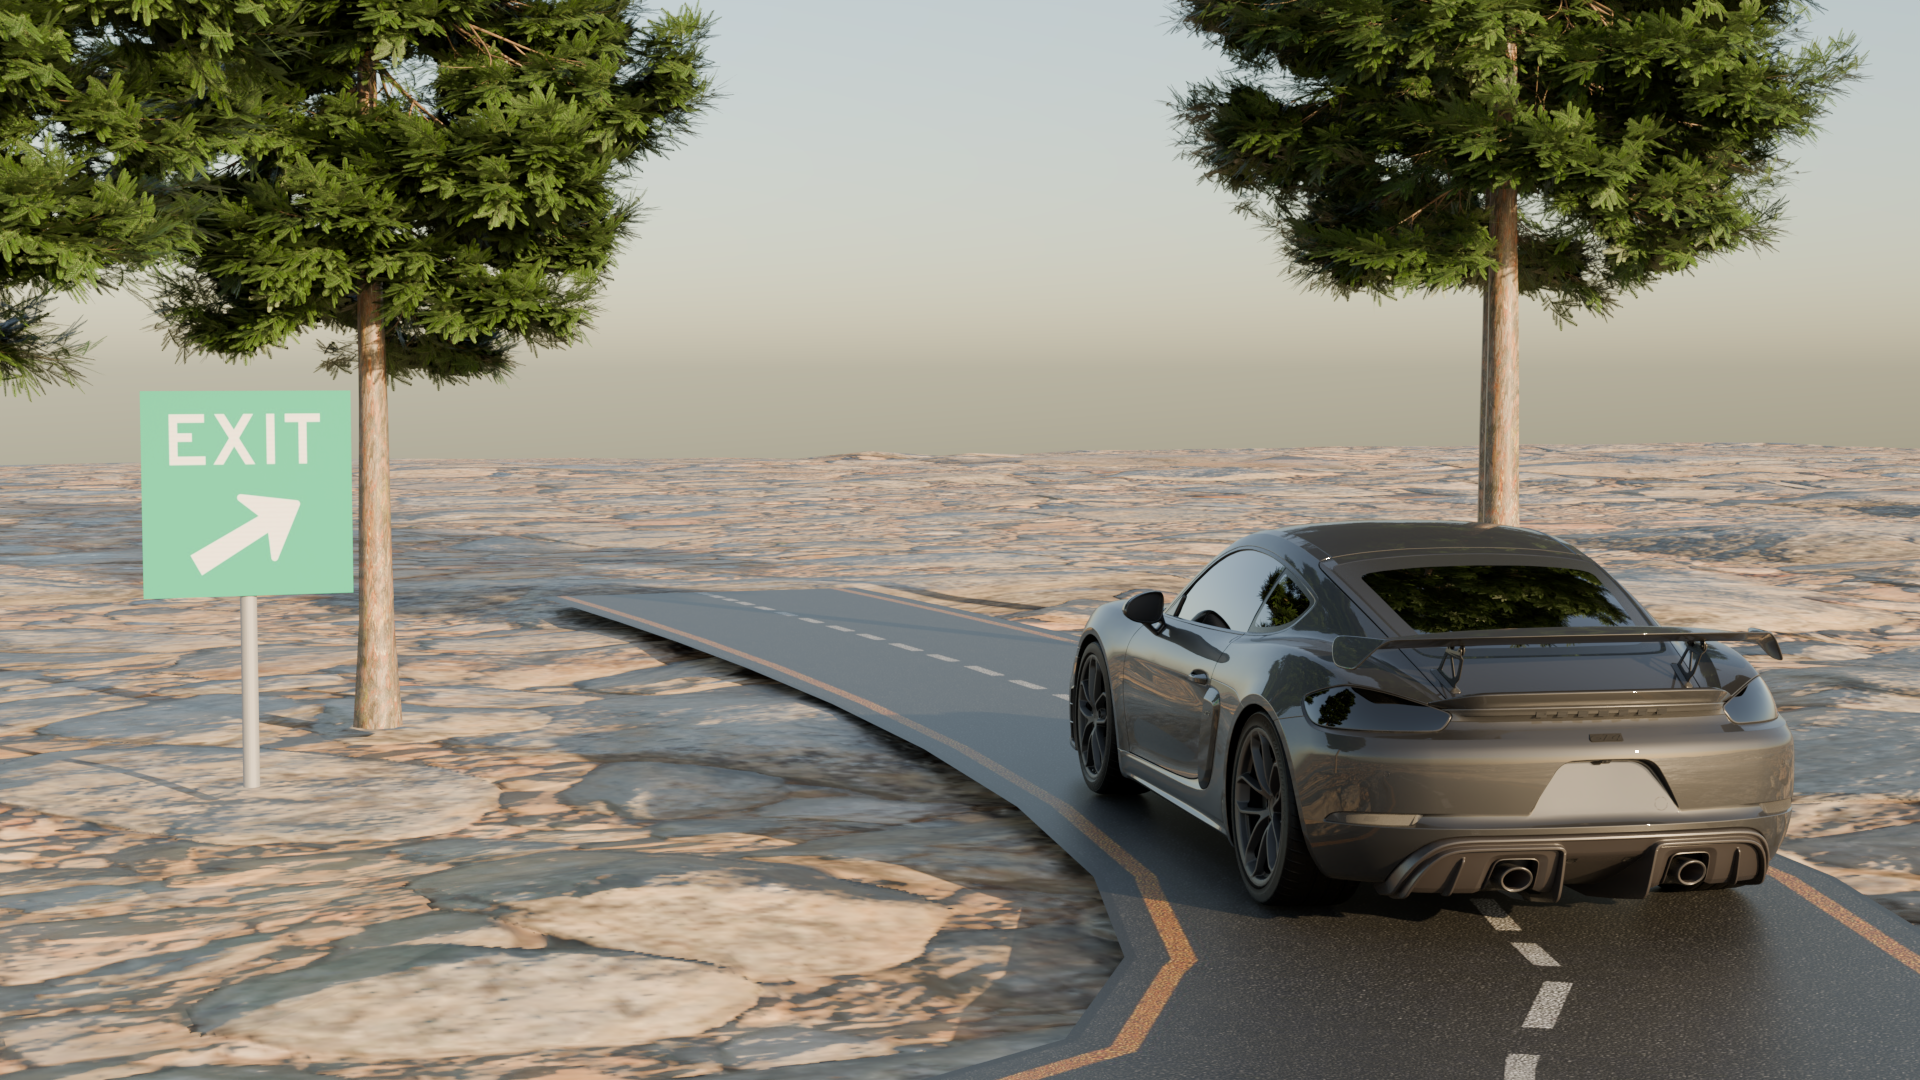
\includegraphics[width=\linewidth]{images/initial_scene.png}
  \caption{    \caption{Initial scene created using app.py}}
  \label{fig:row_of_images}
\end{figure}
 
 From here we focused on making each function more modular so it could be controlled with general numbers and phrases rather than explicitly defining precise coordinates in the Blender world. Functions had to be adjusted to use other objects as reference points so that the end user would not need to know anything about Blender or the size of each object in order to create a realistic scene. We have listed some of these changes below as examples:
 
 \begin{itemize}
     \item \texttt{generate\_forest} replaced \texttt{create\_tree}, spawning a defined number of trees at random locations near the road.
     \item Road and camera positions now defaulted to \texttt{(0, 0, 0)} in the scene to ensure alignment.
     \item The sign was always placed on the right side of the road at a fixed distance.
     \item A background PNG was placed a fixed distance away from the camera to add more realism.
 \end{itemize}
 
 These types of changes set the foundation for the next phase of our project. A more detailed description of the methods used for each aspect of the scene can be found in the methods section. 
 
 
 \section{Headless Scene Generation}
 
 While we had initially considered developing a lightweight UI using Streamlit, this idea was quickly abandoned in favor of a more streamlined and developer-friendly approach. Instead, we created a single entry-point script called \texttt{run.py}, which executes all of our modular scene generation functions in sequence while running Blender in headless mode.
 
 To ensure flexibility and reproducibility, all necessary parameters for a scene generation run are stored in a centralized \texttt{config.json} file. This JSON configuration file includes values for terrain type, sign appearance, weather effects, background selection, lighting conditions, and more. This allowed us to easily adjust scenes without altering the Python code, and also made the generation pipeline more portable and scriptable.
 
 At runtime, \texttt{run.py} loads these parameters from \texttt{config.json}, dynamically builds the scene using the corresponding modules, and exports the rendered images along with COCO-style annotations. This modular structure enables quick iteration and experimentation with various scene setups.
 
 Some key features of this approach include:
 
 \begin{itemize}
     \item Modular components for different scene elements (e.g., \texttt{blender\_road.py}, \texttt{blender\_signs.py}, \texttt{blender\_trees.py}, etc.).
     \item Automatic GPU acceleration setup using Blender's Cycles renderer.
     \item Dynamic camera placement and movement, optimized for capturing objects of interest (e.g., traffic signs).
     \item Procedural asset placement and randomized backgrounds for realistic and diverse outputs.
     \item Built-in support for snow and lighting effects using parameterized controls.
     \item Output image annotations formatted in COCO style for machine learning training and evaluation.
 \end{itemize}
 
 By combining headless execution with configuration-based customization, our scene generation workflow is both efficient and highly extensible.

 \section{Methods}
Blender may be controlled without using a user interface via the Blender Python API, which allows for python scripting to replace traditional blender inputs. As the intention of this tool is to allow users to easily integrate data generation into a deep learning pipeline, all scene generation was created using Blender scripting, with the input being a simple JSON file that a user may adjust within certain presets to adjust various scene variables, listed below. Images are output already correctly labeled, and ready to be added to training datasets. 
\subsection{Signs}
Signs were created by collecting a variety of images of common signs in the United States. These signs were then converted to a portable network graphic (PNG) format with a transparent background. In Blender, the sign is applied to a mesh object such that the background of the object is transparent, leaving only the sign in place. This allows for seamless scaling, as well as allowing the user to prepare any PNG as a sign. In order for more realistic images, various damage states and sign orientations may be randomly applied to the sign. Finally, various weather conditions such as snow and mud may be added to the front of the sign, as obstruction due to environmental factors is common in harsher climates. Signs are placed on a simple pole, and positioned correctly within the scene relative to a camera object. 

\begin{figure}[ht]
    \centering
    \begin{minipage}{0.1\textwidth}
        \centering
        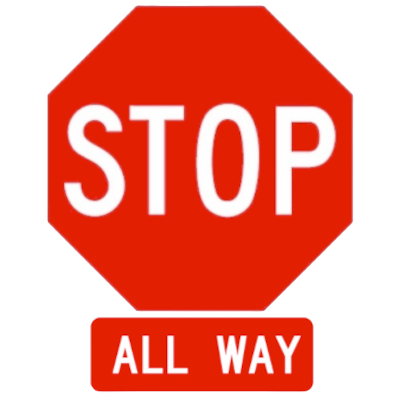
\includegraphics[width=\linewidth]{images/All Way Stop.png}

    \end{minipage}\hfill
    \begin{minipage}{0.1\textwidth}
        \centering
        
\includegraphics[width=\linewidth]{images/Bump.png}

    \end{minipage}\hfill
    \begin{minipage}{0.1\textwidth}
        \centering
        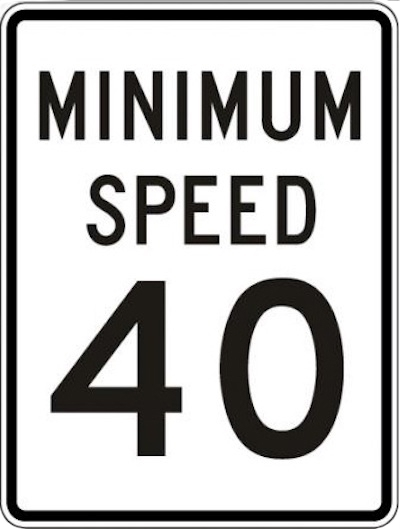
\includegraphics[width=\linewidth]{images/Minimum Speed 40.png}

    \end{minipage}
    \caption{Representative samples of sign input images}
    \label{fig:row_of_images}
\end{figure}

\subsection{Roads}
Preset road scenes were similarly created via Python scripting. A simple two-lane road, as well as a highway scene were constructed using free mesh objects and textures from BlenderKit[XXXX], but could be recreated using a variety of available Blender resources. Roads include concrete barriers, guardrails, lighting, and lane divisions. Optionally, the road was curved in the 3D space, with lane coordinates returned to allow the camera object to move along each lane to correctly imitate real-world roads. 
\subsection{Environment}
Each road was placed on a plane which may be changed between various pre-set images to simulate diverse environments. Similar to the road objects, this plane was randomly curved in the 3D space to match the orientation of the road, effectively simulating topological changes, which affect both camera placement and sign visualization as the camera moves through the simulated scene. Additionally, different weather conditions including snow, rain, and fog were used to expand the dataset to include environmental obstructions of the sign directly within the camera field of view. 

One of the main benefits of using a free platform such as Blender is that there are a wide variety of plugins, both free and paid, which can be used to improve scene creation. Here, a tree add-on was used to generate different styles of trees, which were then randomly scattered in the scene. 

\subsection{Trees}
To add a sense of realism to the scene, we added the option to randomly generate trees on the sides of the road. We used the Sapling Tree Gen blender add-on which was available for free online. Assets and materials used to make the tree look more realistic were obtained for free online from popular material and asset blender add-on 'blenderkit'. We wanted to limit the amount of set up required to begin generating images so the final tree function has limited optionality. These limited options were chosen to give sufficient variety, remain reasonably efficient to render, and to occasionally partially oclude the sign to improve model robustness. 

Presets include: "Many trees," "Some trees," and "No trees" for density; and "Close" or "Far" for distance from the road.

Tree Density:
"No trees" disables tree generation entirely, leaving the sides of the road clear.
"Some trees" generates 16 trees along the road, providing moderate environmental clutter.
"Many trees" doubles the count to 32 trees, increasing realism and the chance that trees may partially obscure the road signs. This supports the goal of improving model robustness to occlusions.

Tree Distance from Road:
"Close" places trees between 15 to 40 units from the road, allowing for potential sign occlusion.
"Far" increases the placement range to 40–100 units, ensuring trees remain purely background elements and do not interfere with the road or signs.

This balance of simplicity and variability allows quick scene generation with enough randomness to train models that generalize better to real-world occlusions and backgrounds.

\subsection{Background Plane} A background plane is employed to simulate realistic environmental elements such as skies, mountains, and urban landscapes. The plane’s texture is randomly chosen from a collection of user-supplied images. The orientation of the plane is dynamically linked to the camera, ensuring the background continuously aligns with the camera's viewpoint and preventing the background from ever going out of frame. Users can easily customize the scene by providing their own images, which are automatically incorporated into the scene, significantly enhancing flexibility and personalization of the generated data.

\subsection{Terrain} Each road scene includes a terrain plane, with textures randomly selected from a folder containing materials formatted according to the Polyhaven specification. The process for applying these textures is automated; users simply place new texture folders into the terrain directory to seamlessly incorporate additional terrain types. Currently available terrains include rocky, snowy, and grassy textures, automatically enhancing the realism and variability of generated scenes.

\subsection{Camera}
Our camera setup aimed to simulate realistic dashcam footage, capturing a vehicle traveling along a roadway while allowing significant flexibility regarding the placement and movement of the camera to create diverse visual scenarios. 

Initially, the camera was a simple object used only to view objects of interest within the scene. Blender offered flexibility in positioning and rotating the camera across the three-dimensional axis, constrained only by the defined Blender world boundaries. The camera was initially placed at fixed x, y, and z coordinates and manually rotated to meet scene requirements. Once the scene was rendered, snapshots of the desired objects, such as traffic signs, were captured.

Camera dynamics were significantly refined as our task evolved to generate more robust synthetic datasets. With the introduction of a single-lane straight road within Blender, the camera was programmatically positioned at the road's starting coordinates and then moved incrementally along this road. At this stage, parameters such as the step movement and the number of steps were manually set and defined as adjustable user inputs within our Python scripts.

To eliminate hardcoded parameters and improve adaptability, we positioned the camera relative to key scene elements and automatically adjusted its orientation to face forward based on contextual cues. This dynamic placement utilized bounding boxes defined around objects to calculate their relative distance from the road's initial coordinates. The camera placement system included multiple initial position options: a Vehicle-Based Placement Option, where the camera positioned itself relative to a vehicle object using presets like behind, in front, above, or simulating the driver's viewpoint; and a Lane-Based Placement Option, placing the camera centrally within a user-selected lane and oriented forward, simulating a vehicle traveling along that lane.

The camera script was further enhanced to accommodate the increasingly complex geometry of the generated roads—such as multi-lane and curved roads. The revised script would allow the camera to begin in any lane and smoothly change course when the geometry of the road changes. Several methods for smooth camera movement along curved roads were explored, including mathematical curve definitions within Blender to simulate realistic dashcam trajectories. Adhering to the principle of Occam's razor, the simplest yet most effective method chosen involved subdividing the road object into multiple segments and generating discrete points along the road for camera placement. Vector-based calculations were used to fine-tune the camera's position and orientation as it moved through the scene. In particular, the direction vector between the camera and the traffic sign was constantly assessed to keep the alignment forward, ensuring smooth transitions and consistent sign visibility throughout the camera's trajectory.

We created a camera controller script to automate controlled, randomized camera movements to generate a dataset methodically. This script dynamically changes the camera's position while maintaining the traffic sign within the camera frame. However, It was challenging to guarantee constant visibility of the sign object as Blender also rendered frames in which the sign was absent. As a solution to this, we automatically skipped all such frames during the rendering process.

Once camera movement was sufficiently addressed, we focused on enhancing camera properties such as lens position, lens type, focal length, and motion blur to emulate realistic dashcam perspectives. These camera property enhancements were partially implemented within Blender's local rendering engine but achieved greater effectiveness during post-processing. Consequently, we created a separate Python script utilizing OpenCV to apply realistic dashcam effects, including motion blur, lens flare, vignette, sensor noise, rolling shutter distortion, and compression artifacts more efficiently and consistently during the post-processing stage.

We also added a bounding box functionality to generate a bounding box around essential objects in the scene, such as traffic signs. Each rendered camera frame included a matching bounding box metadata file to align visual data accurately with ground-truth annotations.

\subsection{Background \& Lightning}
Rendering complex backgrounds directly within the Blender scene proved computationally intensive. We added static images positioned at a fixed distance behind the road as a more efficient alternative. These images were connected to the camera's movement to keep the sky background in our scenes constant.

Lighting was also added via Blender's light object, which allowed for simulations of shadows, reflections, and other lighting aberations, a significant improvement from previous Blender image-generation strategies\cite{blender_paper}. 

\subsection{Weather}
Using Blender's particle system, weather conditions like rain and snow were added to the generated blender scene to increase their realism and resilience.

Snow effects were integrated into the scene using predefined weather condition presets, including light, moderate, and heavy snow and hailstorms. Each preset configured specific particle density, count, sizes, gravity settings, and random movements (Brownian factor) to simulate realistic snowfall. Particles were emitted from a large plane above the scene, with particle lifetime, gravity, and particle randomness adjustments to achieve authentic snowfall dynamics.

The Rainfall effect was simulated through a similar particle system with customizable density settings. Smaller than snow particles, raindrops were released from a plane over the scene with higher gravity settings. Raindrops traveled straight downhill with little random movement, in contrast to snow. The shorter particle lifespan reflected the characteristics of semi-realistic rain.

\subsection{Annotations}
All images were rendered and stored following the Common Objects in Context (COCO) annotation scheme for later ease of use. As the scene variables were carefully controlled, each generated image contains metadata including scene variables as well as a bounding box for the sign within the image. 

\begin{figure}[ht]
    \centering
    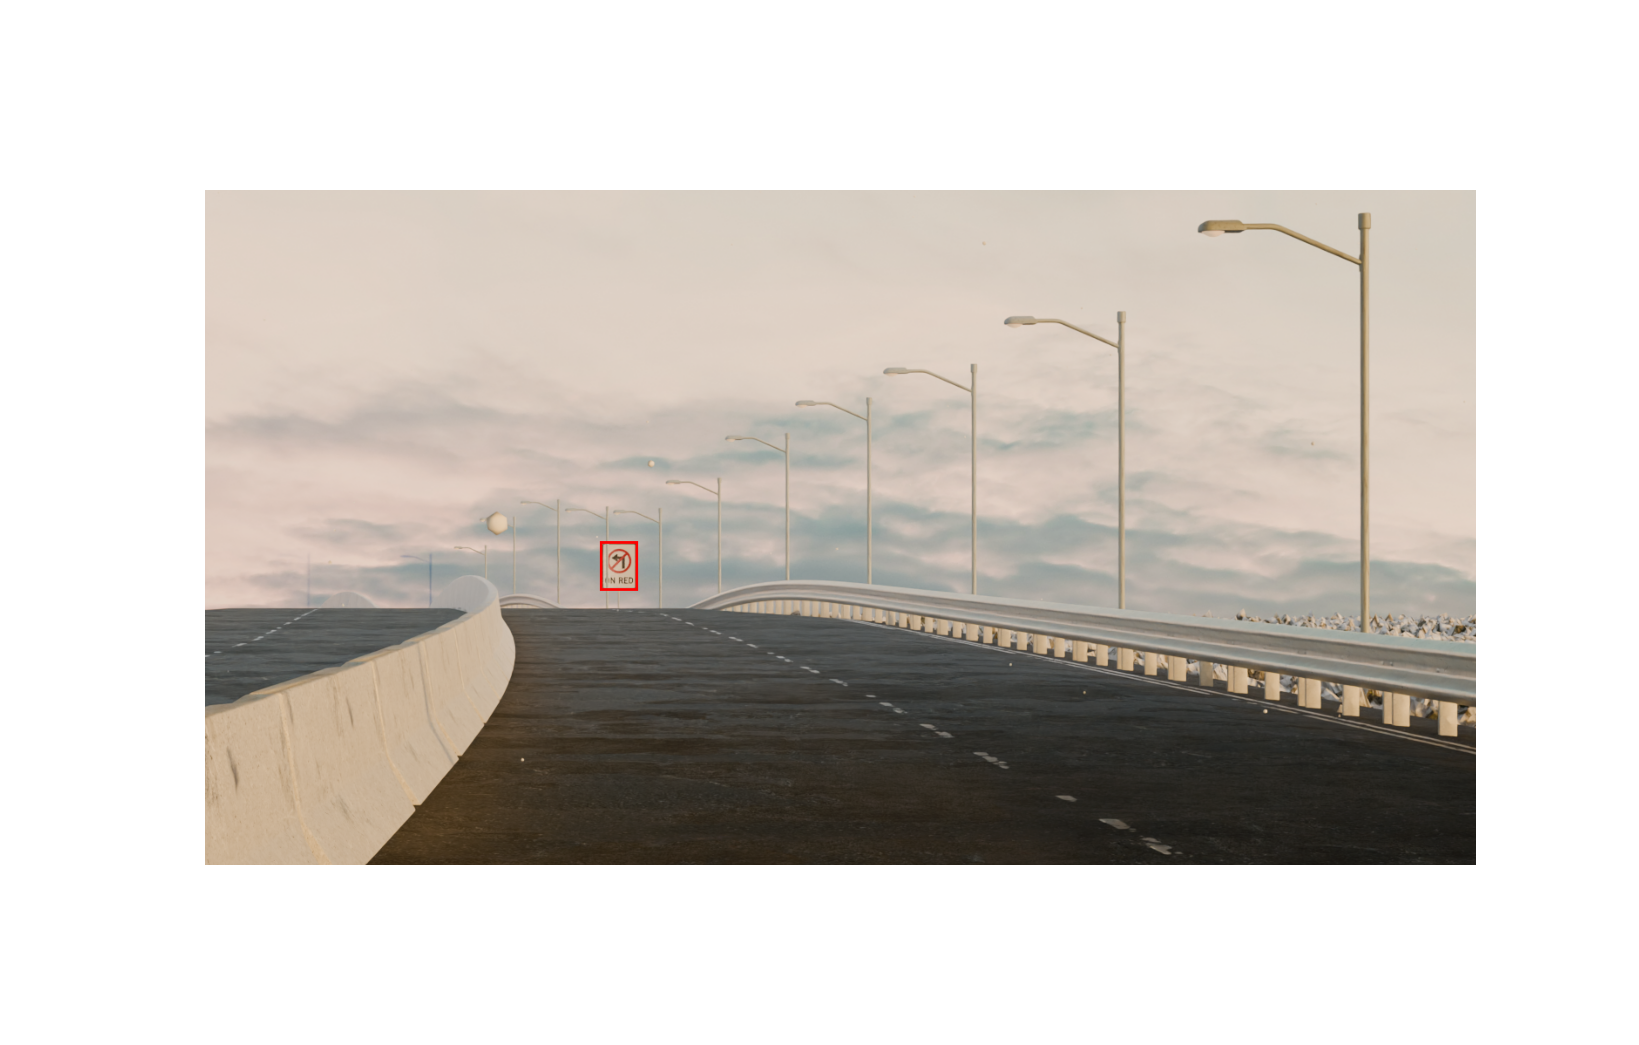
\includegraphics[width=\linewidth]{images/sign w box.png}
    \caption{Sample of generated image, including a red bounding box around the sign}
    \label{fig:row_of_images}
\end{figure}



\subsection{Effect on Real World Datasets}
To evaluate the effect on real world datasets, both DETR \cite{DETR} and YOLO\cite{glenn_jocher_2022_7347926} models were trained with several different datasets. Initially, they were trained with an open source sign dataset (XXXXX), which contained 2817 street signs from various global locations. Next, the models were trained on a completely synthetic dataset containing 3061 images generated using the Blender pipeline outlined here. Finally, the models were trained on a combined dataset containing equal parts synthetic and real data. Each model was tested using a validation set collected from a local neighborhood, with 114 images. 

\section{Data Exploration}
We have three distinct traffic sign datasets:

\subsection{Open Images V7}
A large, public dataset that includes a variety range of traffic sign images and their corresponding annotations. However, very few of those images are taken from a dash-cam view, so their viewpoint differs from our target domain.

\subsection{Synthetic Data}
We generated around 3k synthetic images through Blender script, rendering traffic sign scenes that mimic dash-cam optics (motion blur, road curvature, varying lighting, etc.). This synthetic dataset not only matches the viewpoint we care about but also save our time and cost to collect data.

\begin{figure}[h]
    \centering
    %----------- Open Images V7 ------------------
    \begin{subfigure}[t]{0.48\linewidth}
        \centering
        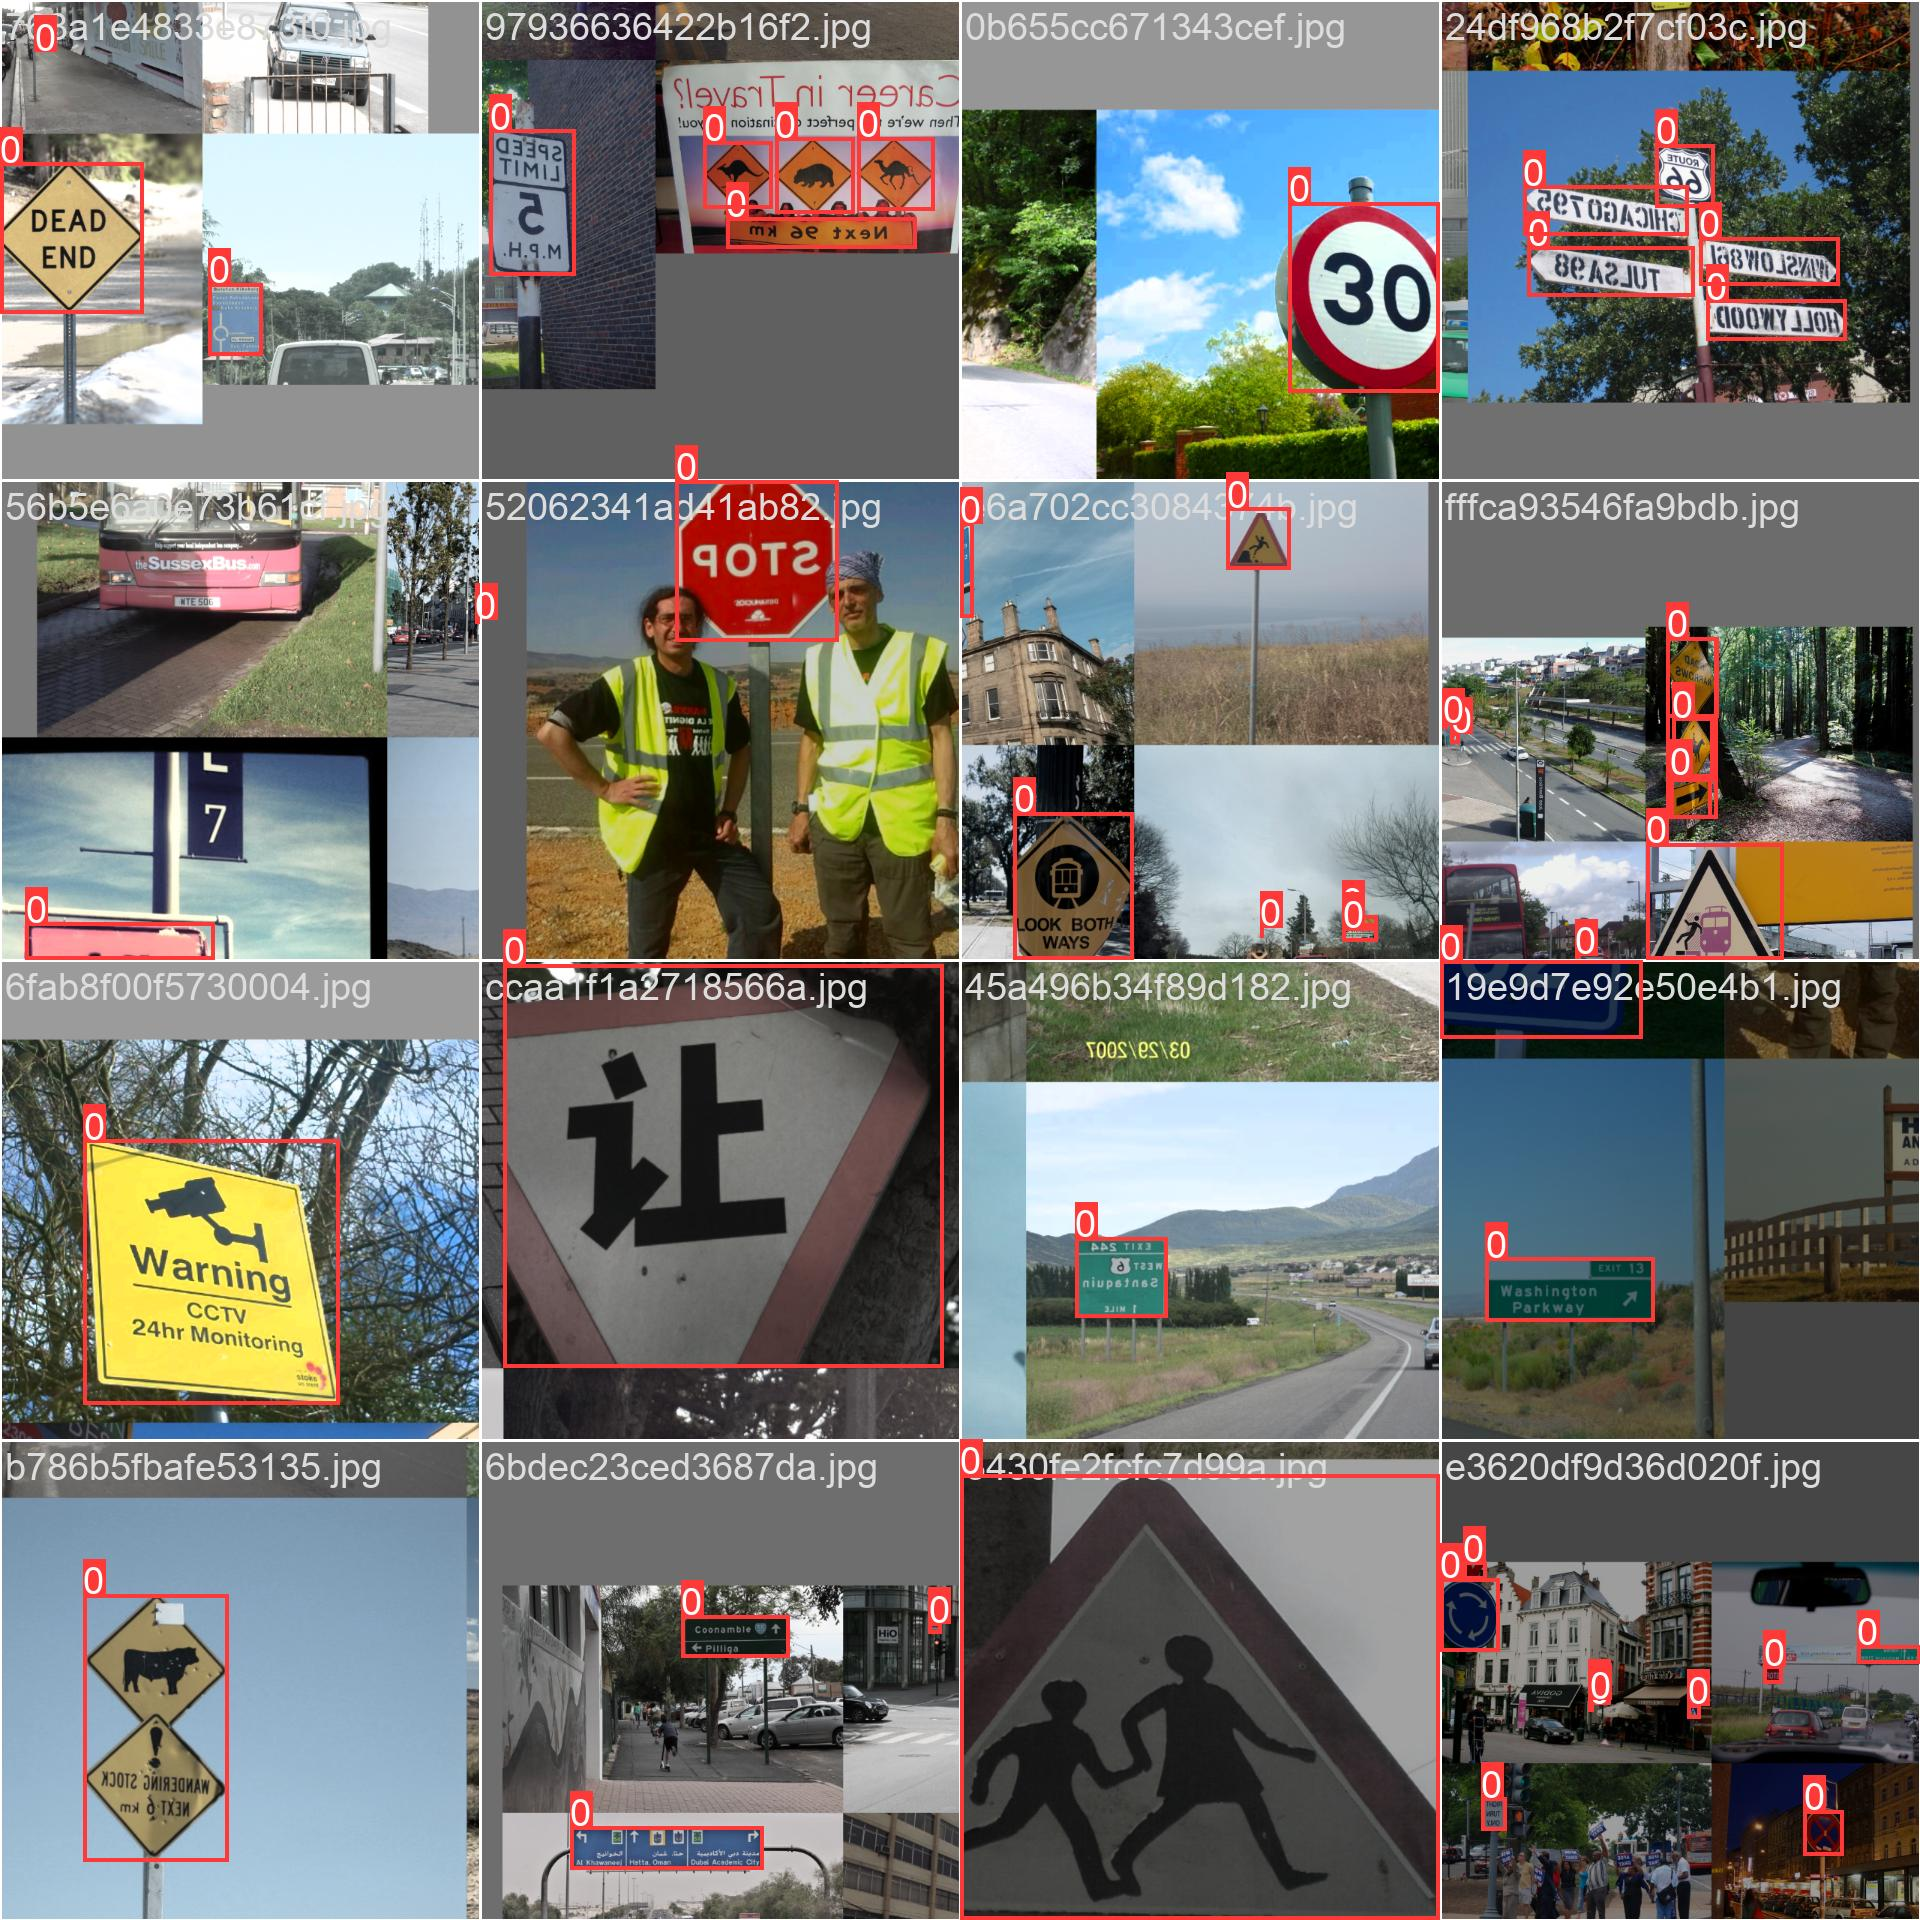
\includegraphics[width=\linewidth]{images/open_source.jpg}
        \caption{Open Images V7}
        \label{fig:open_images}
    \end{subfigure}\hfill
    %----------- Synthetic -----------------------
    \begin{subfigure}[t]{0.48\linewidth}
        \centering
        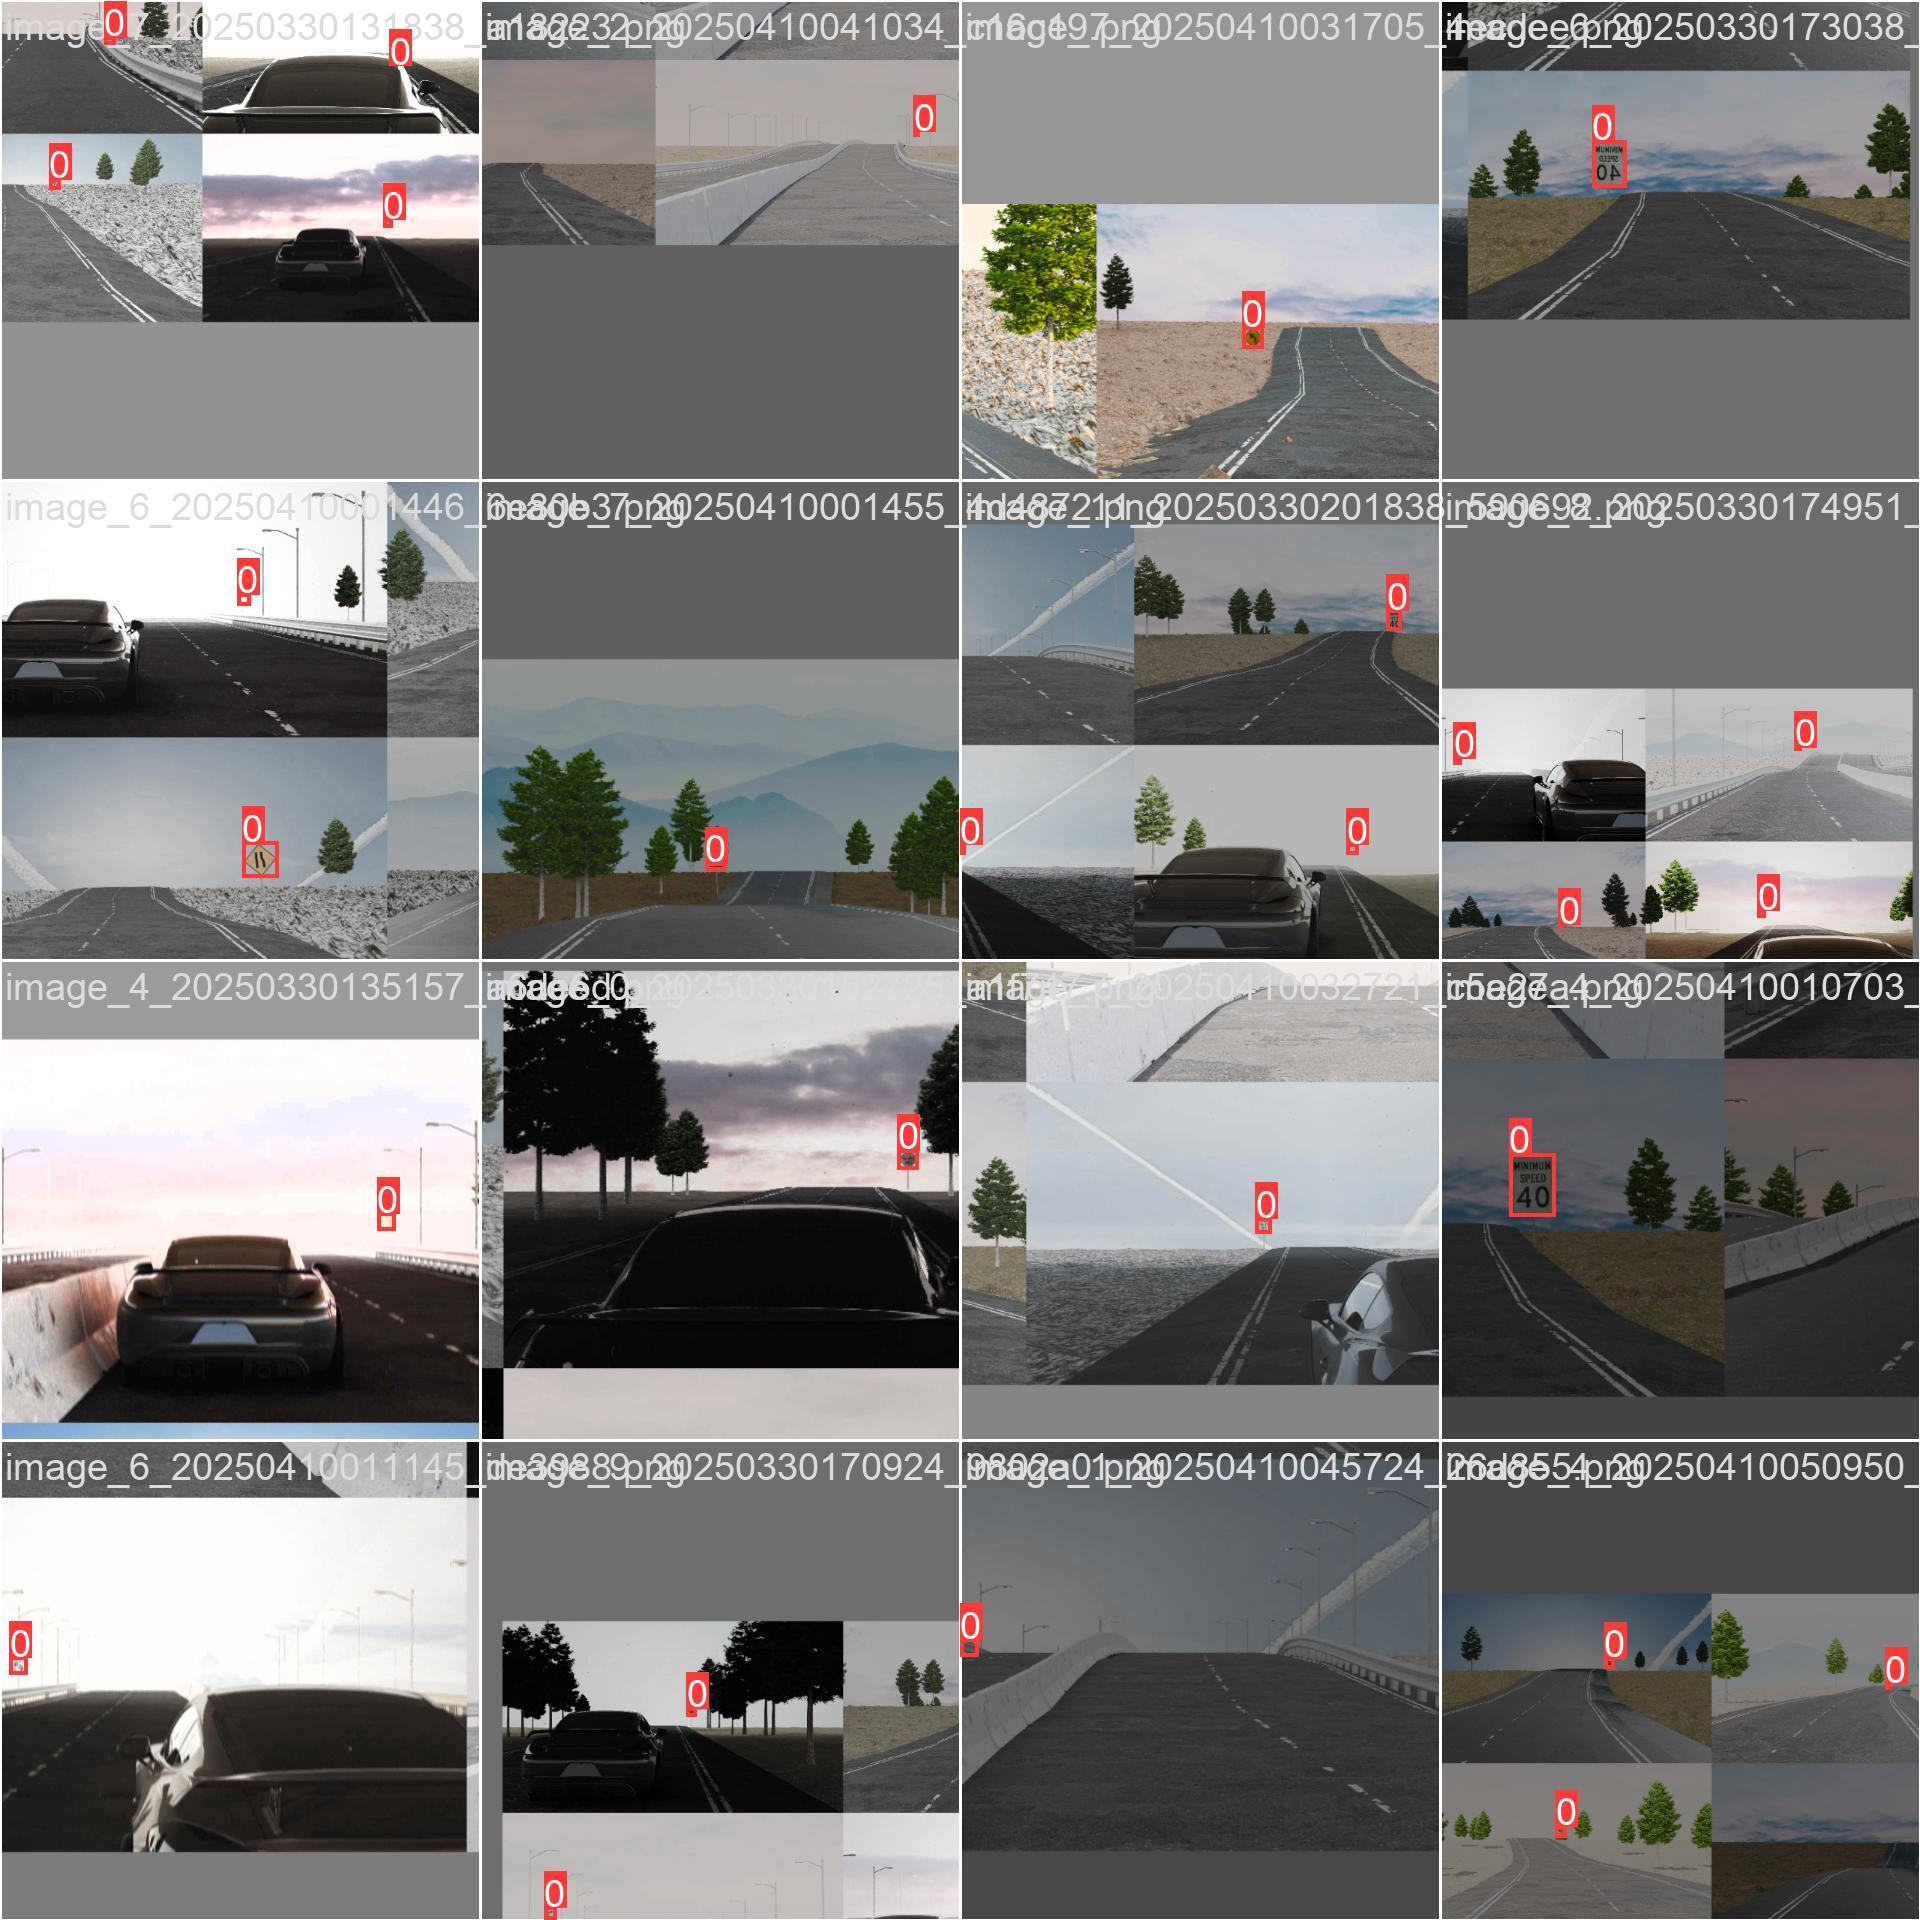
\includegraphics[width=\linewidth]{images/synthetic.jpg}
        \caption{Synthetic (Blender‑rendered)}
        \label{fig:synthetic}
    \end{subfigure}

    \caption{Representative samples from the two training datasets used in this study.}
    \label{fig:datasets_overview}
\end{figure}

\subsection{Blyncsy Data}
Provided by Blyncsy, a Utah-based transportation-analytics company, and used for validation. This collection consists of real dash-cam images captured on roads and professionally annotated.

\begin{figure}[h]
    \centering
    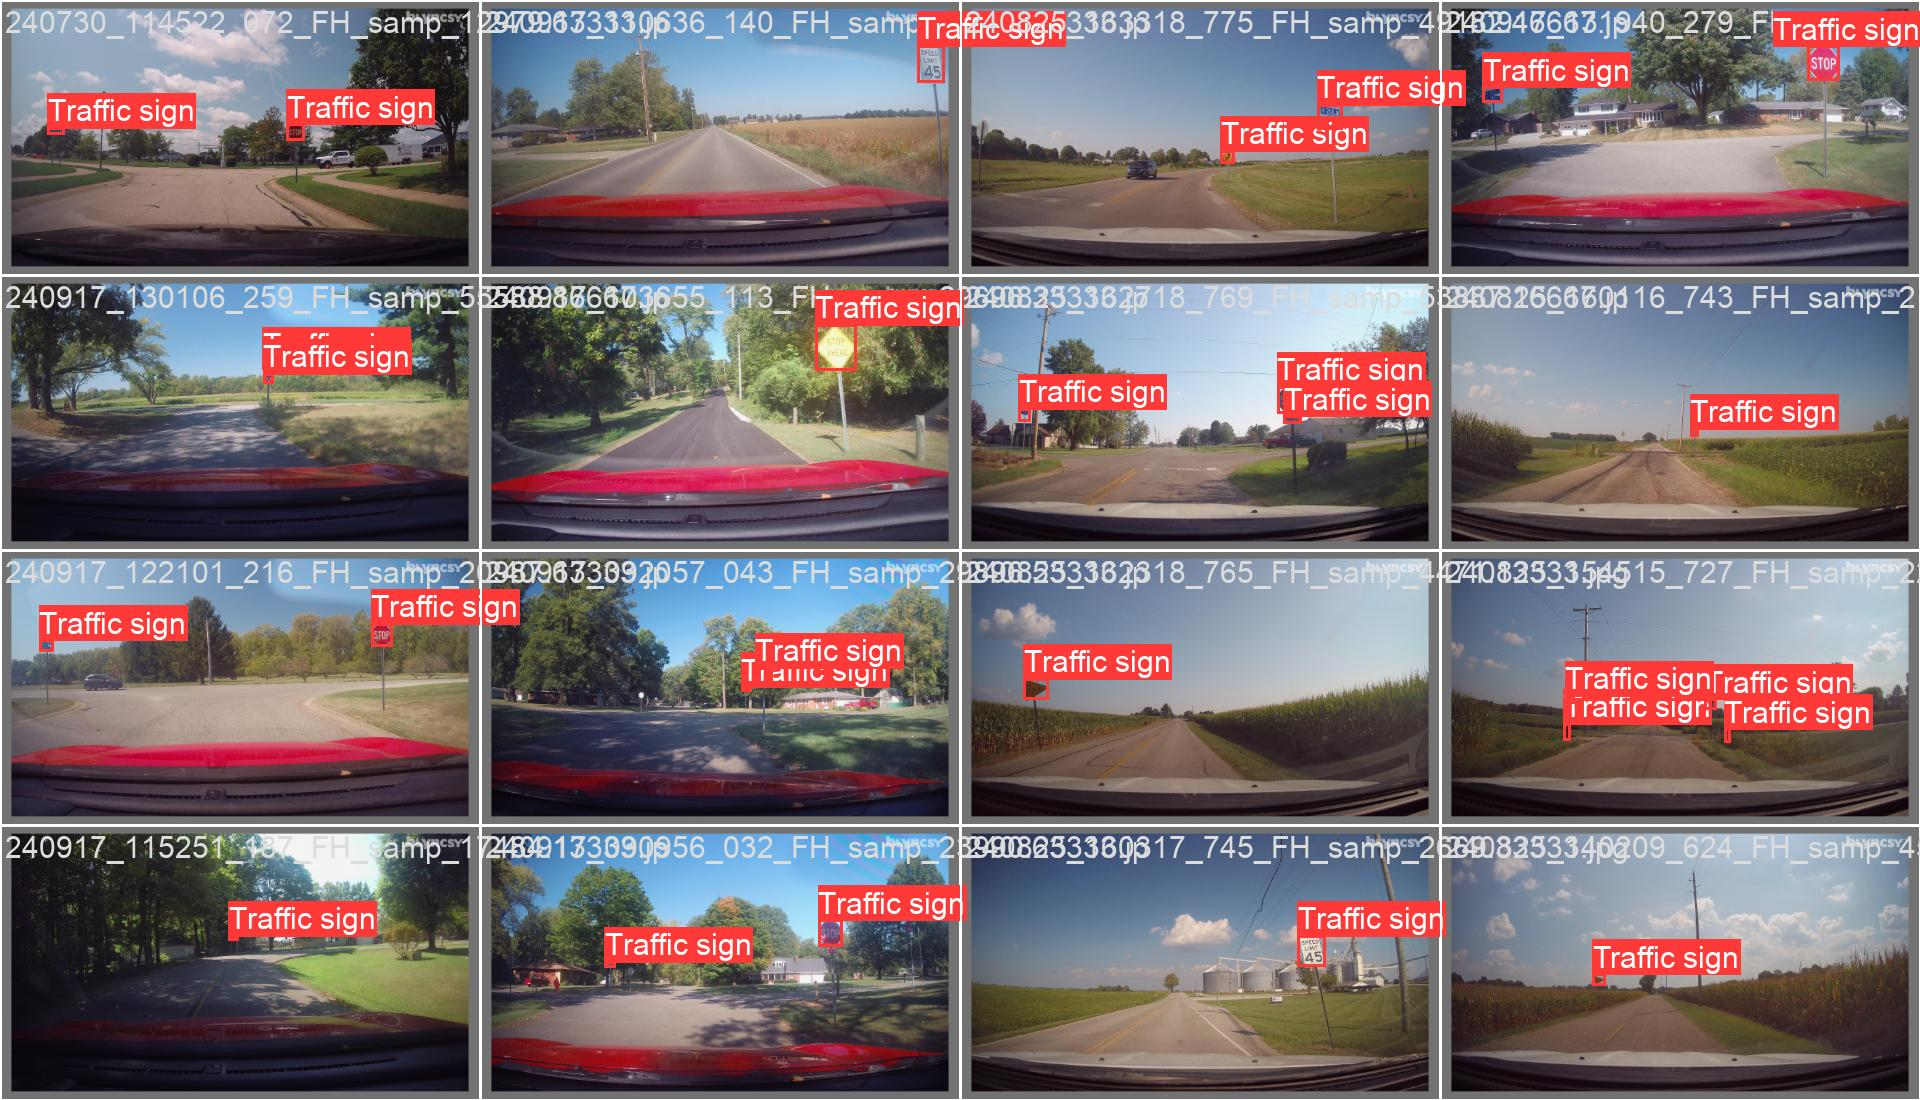
\includegraphics[width=\linewidth]{images/dashcam.jpg}
    \caption{Samples of validation dataset}
    \label{fig:row_of_images}
\end{figure}

\section{Methods Exploration}
%TO DO: Show generated images, train a model on a known dataset, train with just our dataset, and a combined dataset to show metrics
Detecting and recognizing traffic signs from dash-cam views is essential for companies like Blyncsy, which support cities and state Departments of Transportation in automating roadway maintenance and asset inventory tasks. However, this task presents numerous challenges: the camera is constantly in motion, traffic signs often occupy only a small fraction of the frame, lighting and weather conditions can change abruptly, and signs are frequently occluded by foreground objects. Bridging this "viewpoint gap" typically requires large, well-curated dash-cam datasets—resources that remain scarce in the public domain.

Using a Blender script, we can efficiently render thousands of synthetic, dash-cam-style images within a few hours. These images can be generated with varied sign types, distances, lighting conditions, weather, motion blur, and backgrounds. Despite this, it remains uncertain to what extent such synthetic data can enhance a model’s ability to detect traffic signs.

In this study, we conduct a controlled investigation using YOLOv5 and DETR to address a straightforward question: How will the synthetic data affect the performance of traffic sign detection model? To answer this, we train three models separately under the same hyperparameter settings:

\begin{enumerate}
  \item \textbf{Open‑source only}: real images from the Open Images V7 traffic sign subset ($\approx3\,k$).
  \item \textbf{Synthetic only}: dash‑cam views from Blender script ($\approx3\,k$).
  \item \textbf{Combined}: Combine the above two datasets ($\approx6\,k$).
\end{enumerate}

\subsection{YOLOv5}
YOLOv5 is an efficient and widely adopted one-stage object detector, well known for its speed, accuracy, and simple deployment \cite{glenn_jocher_2022_7347926}. In our experiment, we employed the YOLOv5s architecture and maintained identical hyperparameter settings across all three training regimes to ensure a fair and controlled comparison.

To prepare our synthetic dataset for training, we first needed to convert its bounding box annotations into the YOLOv5 format. Initially, our annotation files recorded bounding boxes using top-left corner coordinates along with height and width. However, YOLOv5 expects bounding boxes in a different structure: the $(x, y)$ coordinates of the bounding box center followed by the width and height, all normalized with respect to image dimensions. We implemented a preprocessing step to convert each annotation accordingly, ensuring compatibility with YOLOv5’s training pipeline.

Each model was trained for 10 epochs. All input images were resized to 640×640, and we kept the learning rate, data augmentation policies, and confidence thresholds consistent across experiments. Performance was evaluated on the Blyncsy validation set, which consists of real dash-cam images.

As shown in Table~\ref{tab:model_comparison}, the model trained on the combined dataset (Model 3) achieved the best overall performance, recording the highest values for mAP@0.5, mAP@0.5:0.95, and recall. This indicates that leveraging both real and synthetic data allows the model to benefit from the specific knowledge of the synthetic data while retaining the realism of real images. Model 1, trained solely on real images data, followed closely and achieved the highest precision, suggesting real images can avoid false positives.

In contrast, Model 2, trained only on synthetic data, significantly underperformed across all metrics. While it achieved moderate precision, its low recall and mAP values indicate limited generalization to real-world images. This suggests that synthetic data alone lacks sufficient realism, though it can still provide useful clues under high-confidence thresholds.

These findings indicate that although synthetic data alone may not be sufficient for robust real-world performance, it is highly valuable when used to augment real datasets. By simulating the dash-cam view and enabling large-scale generation at low cost, synthetic data helps improve the domain gap.



\begin{table}[ht]
\centering
\begin{tabular}{|l|c|c|c|}
\hline
\textbf{Metric} & \textbf{Model 1} & \textbf{Model 2} & \textbf{Model 3} \\
\hline
mAP@0.5 & 0.768 & 0.375 &  \textbf{0.788}\\
mAP@0.5:0.95 & 0.512 & 0.19 & \textbf{0.526}\\
Recall & 0.654 & 0.346 & \textbf{0.705}\\
Precision & \textbf{0.844} & 0.671& 0.811 \\
\hline
\end{tabular}
\caption{Comparison of three yolov5s models' performance metrics.}
\label{tab:model_comparison}
\end{table}

\subsection{DETR - Detection Transformer}
DEtection TRansformer (DETR) is a transformer-based object detection model that reformulates object detection as a direct set prediction problem. Unlike traditional detectors, DETR eliminates the need for anchor boxes and non-max suppression by using a global attention mechanism to directly predict object positions and classes. Though computationally heavier, DETR has been shown to perform well on tasks requiring structured reasoning and benefits from longer training durations.

For this study, we used the standard DETR architecture and followed the same experimental setup as described for YOLOv5, using the same dataset splits and identical data preprocessing pipelines. Bounding box annotations were converted from the original top-left format to the required format expected by DETR, with normalized coordinates and class labels. To account for DETR’s slower convergence, we trained each model for 60 epochs, compared to 10 for YOLOv5.

Performance was evaluated using the COCO-style evaluation metrics on the Blyncsy validation set. As shown in Table~\ref{tab:detr_model_comparison}, the model trained on the combined dataset (Model 3) again outperformed both other configurations across all key metrics. It achieved the highest overall mAP (0.31), the best mAP@0.5 (0.608), and the highest recall (0.405), consistent with the YOLOv5 results. This suggests that combining real and synthetic data also improves performance for transformer-based models, not just convolutional ones.

Model 1, trained exclusively on real images, performed reasonably well and achieved competitive scores, especially in terms of AP@0.5. Model 2, trained only on synthetic images, lagged behind the others in all aspects, reinforcing the earlier finding that synthetic data alone is not sufficient to ensure generalization to real-world traffic sign imagery.

These results further support the conclusion that synthetic data, while less effective on its own, provides meaningful value when integrated with real-world datasets. The consistent performance gains seen in both DETR and YOLOv5 underscore the benefit of leveraging synthetic dash-cam imagery for enhancing traffic sign detection models.

\begin{table}[ht]
\centering
\begin{tabular}{|l|c|c|c|}
\hline % Top rule
\textbf{Metric} & \textbf{Model 1} & \textbf{Model 2} & \textbf{Model 3} \\
\hline % Rule below header
AP@[IoU=0.50:0.95] & 0.292 & 0.179 & \textbf{0.310} \\
AP@[IoU=0.50] (mAP@0.5) & 0.581 & 0.402 & \textbf{0.608} \\
AR@[IoU=0.50:0.95, maxDets=100] & 0.376 & 0.235 & \textbf{0.405}\\
AP@[IoU=0.50:0.95, large objects] & 0.491 & 0.326 & \textbf{0.537} \\
\hline % Bottom rule (added for consistency)
\end{tabular}
\caption{Comparison of DETR model performance metrics.}
\label{tab:detr_model_comparison}
\end{table}
\section{Limitations}
While promising, the methods and results outlined here have several important limitations. Perhaps the most critical being the currently limited scenes that are being generated. No city-scapes, complex roads, or difficult terrain is being synthesized here. However, the framework for such expansions has been clearly layed out. The improvement to model performance demonstrated with a relatively limited range of scenes, however, is encouraging and suggests wide applicability to model improvement, particularly when more targeted scene creation is employed. Similarly, the complexity of the scenes is currently minimal, especially when compared to existing simulation software such as CARLA. Our team attempted to utilize CARLA to generate training images, but ultimately abandoned that route due to the complexity of sign generation and placement within CARLA's synthetic scene. However, images obtained from CARLA are almost certainly more realistic than those generated with our blender pipeline, and future work should include an investigation of how best to merge synthetic outputs. Currently, the sign models created in Blender may be exported to be used in other synthetic data frameworks, as needed.


\section{Conclusion}
As signs are critical to safe and efficient roadways, it is important that detection models can quickly and correctly adapt to new road signs or specific signs. Synthetic data, generated using a free Blender pipeline, provides a fast and effective way to augment existing image datasets for better model performance.

Our results show that the model trained on the combined dataset achieved the highest mAP@0.5, mAP@0.5:0.95, and recall, indicating strong overall performance and effective generalization across data. While the model trained solely on real images (Model 1) achieved the highest precision, its slightly lower mAP and recall suggest that it may be more conservative in detections. In contrast, the model trained only on synthetic data (Model 2) significantly underperformed in both mAP and recall, though it still maintained a high precision, highlighting its potential for producing accurate but sparse detections in specific scenarios.

These findings indicate that synthetic data alone may not be sufficient to train a robust model for real-world deployment. However, when used in combination with real data, it becomes highly valuable by introducing viewpoint consistency, reducing domain gaps, and significantly lowering the cost and effort of data collection and annotation.

In summary, we are confident that our synthetic data generation pipeline not only enhances traffic sign detection models but also lays the foundation for broader roadway applications, including sign size estimation, road damage detection, and analysis of environmental conditions.

\section{Future Work}
While our experiments validate the effectiveness of combining synthetic and real data for traffic sign detection, there are several directions for future work to improve realism and model performance.

One major area is improving the diversity of synthetic data. Currently, every scene contains only one road and one traffic sign. In the future, we will introduce more complex layouts, such as intersections and urban street scenes. Also, we plan to generate multiple traffic signs in each scene, including overlapping or occluded signs, to better mimic real-world situations.

Additionally, we can improve the post-processing and data-cleaning pipeline. Currently, raw output often includes similar images or misplaced objects. Automating post-processing and quality control will ensure that the dataset is consistently usable and reduces the risk of hampering the model performance.

Finally, we plan to develop a post-processing pipeline to clean the generated images. This includes automatically filtering out low-quality or redundant images, and correcting object placement errors. In order to ensure high-quality and diverse training data, we aim to maximize the utility of synthetic data and improve the performance of the model. The above enhancements will make the dataset more reliable and scalable.


% use section* for acknowledgment
\section*{Acknowledgment}


Sridhar, U of U Deep Learning Certificate program, state of Utah.... 


% Can use something like this to put references on a page
% by themselves when using endfloat and the captionsoff option.
\ifCLASSOPTIONcaptionsoff
  \newpage
\fi



% trigger a \newpage just before the given reference
% number - used to balance the columns on the last page
% adjust value as needed - may need to be readjusted if
% the document is modified later
%\IEEEtriggeratref{8}
% The "triggered" command can be changed if desired:
%\IEEEtriggercmd{\enlargethispage{-5in}}

% references section

% can use a bibliography generated by BibTeX as a .bbl file
% BibTeX documentation can be easily obtained at:
% http://mirror.ctan.org/biblio/bibtex/contrib/doc/
% The IEEEtran BibTeX style support page is at:
% http://www.michaelshell.org/tex/ieeetran/bibtex/
%\bibliographystyle{IEEEtran}
% argument is your BibTeX string definitions and bibliography database(s)
%\bibliography{IEEEabrv,../bib/paper}
%
% <OR> manually copy in the resultant .bbl file
% set second argument of \begin to the number of references
% (used to reserve space for the reference number labels box)
% \begin{thebibliography}{1}

% \bibitem{IEEEhowto:kopka}
% H.~Kopka and P.~W. Daly, \emph{A Guide to \LaTeX}, 3rd~ed.\hskip 1em plus
%   0.5em minus 0.4em\relax Harlow, England: Addison-Wesley, 1999.

% \end{thebibliography}
{\small
\bibliographystyle{unsrt}
\bibliography{bibtex/bib/bibliography}
}
% biography section
% 
% If you have an EPS/PDF photo (graphicx package needed) extra braces are
% needed around the contents of the optional argument to biography to prevent
% the LaTeX parser from getting confused when it sees the complicated
% \includegraphics command within an optional argument. (You could create
% your own custom macro containing the \includegraphics command to make things
% simpler here.)
%\begin{IEEEbiography}[{\includegraphics[width=1in,height=1.25in,clip,keepaspectratio]{mshell}}]{Michael Shell}
% or if you just want to reserve a space for a photo:

% \begin{IEEEbiography}{Michael Shell}
% Biography text here.
% \end{IEEEbiography}

% % if you will not have a photo at all:
% \begin{IEEEbiographynophoto}{John Doe}
% Biography text here.
% \end{IEEEbiographynophoto}

% % insert where needed to balance the two columns on the last page with
% % biographies
% %\newpage

% \begin{IEEEbiographynophoto}{Jane Doe}
% Biography text here.
% \end{IEEEbiographynophoto}

% You can push biographies down or up by placing
% a \vfill before or after them. The appropriate
% use of \vfill depends on what kind of text is
% on the last page and whether or not the columns
% are being equalized.

%\vfill

% Can be used to pull up biographies so that the bottom of the last one
% is flush with the other column.
%\enlargethispage{-5in}



% that's all folks
\end{document}